\documentclass[border=10pt]{standalone}

\usepackage{tikz}
\usepackage{tikzsymbols}
\usetikzlibrary{calc,patterns,shapes.geometric}

\def\centerarc[#1](#2)(#3:#4:#5){\draw[#1] ($(#2)+({#5*cos(#3)},{#5*sin(#3)})$) arc (#3:#4:#5);}

\begin{document}
	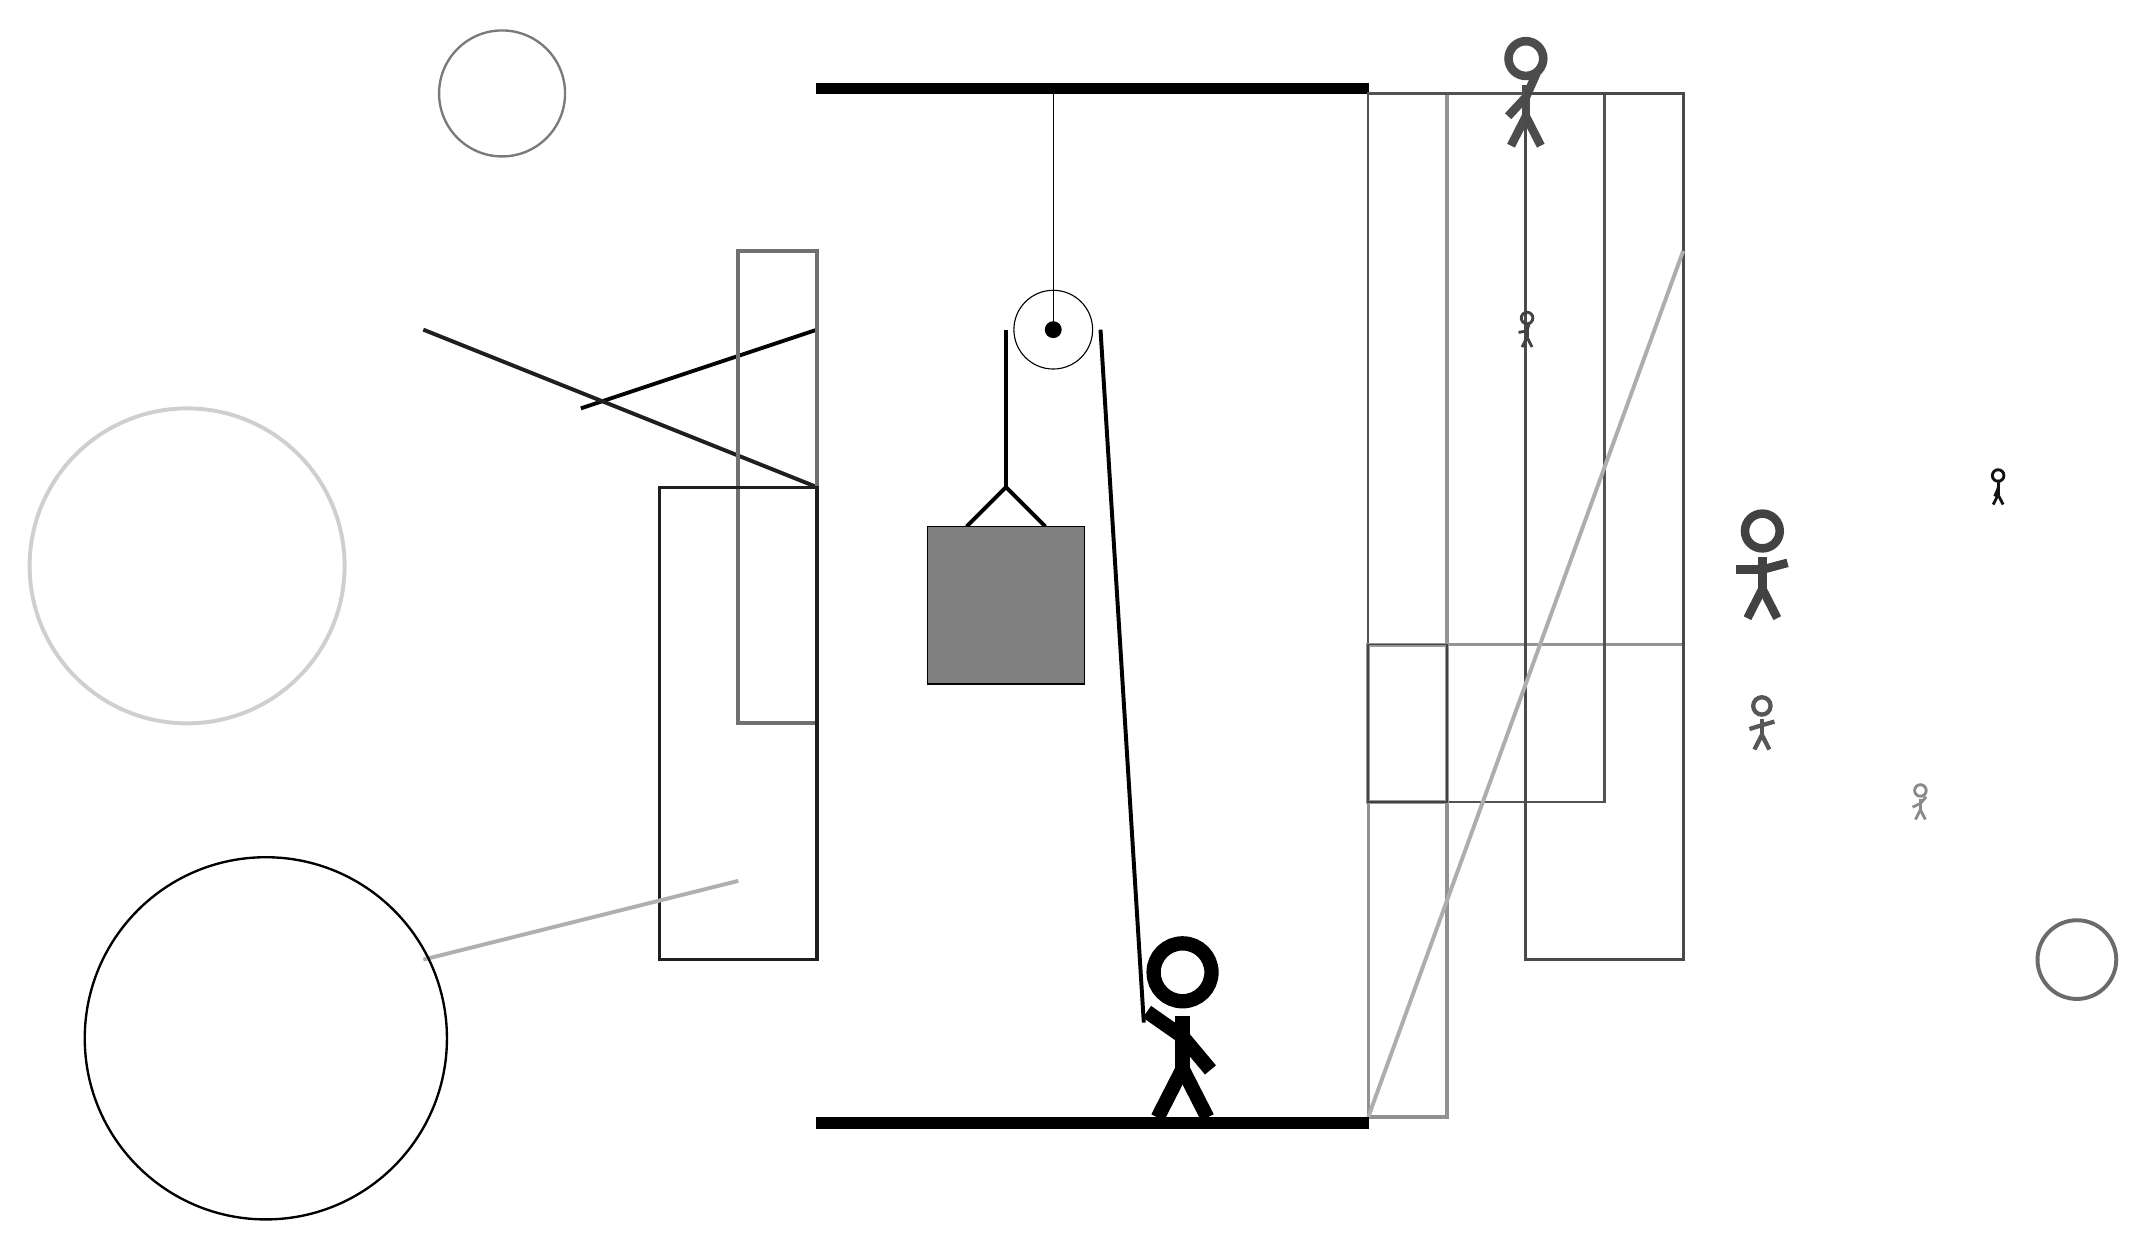
\begin{tikzpicture}
		%%%%% START %%%%%
		
		\draw[fill=black] (-2, 10) rectangle (5, 10.125);
		
		\draw (1, 7) circle (0.5);
		\draw[fill=black] (1, 7) circle (0.1);
		\draw (1, 10) -- (1, 7);
		
		\draw[line width=0.5mm] (-0.1, 4.5) -- (0.4, 5.0) -- (0.9, 4.5);
		\draw[fill=black!50] (-0.6, 4.5) rectangle (1.4, 2.5);
		
		\draw[line width=0.5mm, color=black!99](-2, 7) -- (-5, 6);
		
		\node[line width=0.7mm, color=black!70] at (7, 10) {\Strichmaxerl[6][47][66]};
		\draw[line width=0.5mm, color=black!88](-2, 5) -- (-7, 7);
		\draw [line width=0.3mm, color=black!52](-6, 10) circle (0.8);
		\draw[line width=0.5mm, color=black!56] (-2, 2) rectangle (-3, 8);
		
		\draw[line width=0.4mm, color=black!42] (6, 3) rectangle (9, 10);
		
		\draw[line width=0.3mm, color=black!68] (5, 10) rectangle (8, 1);
		\node[line width=0.4mm, color=black!74] at (10, 4) {\Strichmaxerl[6][0][15]};
		\draw[line width=0.4mm, color=black!43] (5, -3) rectangle (6, 1);
		
		\draw [line width=0.5mm, color=black!58](14, -1) circle (0.5);
		
		\draw[line width=0.4mm, color=black!71] (7, 10) rectangle (9, -1);
		\draw[line width=0.5mm, color=black!77](6, 6) -- (6, 6);
		\node[line width=0.2mm, color=black!66] at (10, 2) {\Strichmaxerl[3][17][16]};
		
		\draw[line width=0.5mm, color=black!32](9, 8) -- (5, -3);
		\draw[line width=0.4mm, color=black!88] (-2, 5) rectangle (-4, -1);
		\draw[line width=0.5mm, color=black!31](-7, -1) -- (-3, 0);
		
		\draw [line width=0.5mm, color=black!19](-10, 4) circle (2.0);
		\node[line width=0.7mm, color=black!93] at (13, 5) {\Strichmaxerl[2][67][84]};
		\draw [line width=0.3mm, color=black!100](-9, -2) circle (2.3);
		\node[line width=0.4mm, color=black!74] at (7, 7) {\Strichmaxerl[2][10][75]};
		\draw[line width=0.5mm, color=black!40] (5, 3) rectangle (6, 1);
		\draw [line width=0.3mm, color=black!61](-2, 6) circle (0.0);
		\node[line width=0.4mm, color=black!46] at (12, 1) {\Strichmaxerl[2][26][49]};
		\draw[line width=0.2mm, color=black!74] (6, 1) rectangle (5, 3);
		
		\draw[line width=0.5mm] (0.4, 7) -- (0.4, 5.0);
		\centerarc[line width=0.5mm](1, 7)(0:180:0.6);
		\draw[line width=0.5mm](1.6, 7) -- (2.15, -1.8);
		
		\node at (2.6, -1.9) {\Strichmaxerl[10][-35][-50]};
		
		\draw[fill=black] (-2, -3) rectangle (5, -3.15);
		
		%%%%% END %%%%%
	\end{tikzpicture}
\end{document}